\documentclass[9pt]{beamer-control}
\usepackage{beamer-control-prac}
\begin{document}
\TOPIC[3]{Frequency Domain}
\CONCEPT[6]{Week 6: Frequency domain analysis}

\begin{frame}
\frametitle{Introduction}
In this practical we will implement a PID controller tuned using the natural frequency and damping ratio of the compound pendulum system, and then perform a frequency domain analysis using Bode and Nyquist plots.

\vfill

This practical will consist of the following parts:
\begin{itemize}
\item PID controller around a pole placement controller
\item Theoretical analysis
\item Experimental analysis
\end{itemize}
\end{frame}

\SUBCONCEPT{PID controller around a pole placement controller}

\begin{frame}{Transfer function}
The closed-loop transfer function for the pole-placement-controlled plant from Practical 5 can be linearly approximated as 
\[
G_{CL}(s)=
\frac{k\omega_n^2}
{s^2+2\zeta\omega_n s+\omega_n^2}
\]
where $k$ is the DC gain, $\omega_n$ is the natural frequency, and $\zeta$ is the damping ratio. For the compound pendulum system, the DC gain is the ratio of the steady-state output angle in radians to the input voltage,
\[
k = \frac{\theta_{\mathrm{ss}}}{V_{\mathrm{in}}}.
\]
As the physical system is nonlinear, the DC gain varies with the operating point. Therefore, the chosen DC gain should be determined at an operating point representative of the expected operating range.
\end{frame}

\begin{frame}{Transfer Function Assessment}
In this procedure you build upon your Simulink block diagram from Practical 5. Our aim is to determine whether the transfer function $G_{CL}(s)$ provides an appropriate model of our pole-placement-controlled system.
\begin{enumerate}
	\item Create a subsystem, including the QUBE and pole-placement controller, in order to simplify your Simulink block diagram.
\begin{figure}	
    \centering
	
\includegraphics[width=8cm]{prac6_pp_subsystem.PNG}
	\caption{Creation of a Simulink subsystem by highlighting a region of the block diagram, right clicking, then creating from selection.}
\end{figure}  
\end{enumerate}
\end{frame}

\begin{frame}{Transfer Function Assessment}
\begin{enumerate}
    \setcounter{enumi}{1}
	\item Apply a Step input of $0.5$V into your new subsystem, which will approximately achieve an angle of $\pi/8$ radians. Use the exact $\theta_{\mathrm{ss}}$ value for calculating $k$, as shown in the figure below.
\begin{figure}	
    \centering
	
\includegraphics[width=6cm]{prac6_dc_gain.PNG}
    
\includegraphics[width=9cm]{prac6_dc_gain_scope.PNG}
	\caption{Finding a DC gain from a voltage input and angle output.}
\end{figure}  
\end{enumerate}
\end{frame}

\begin{frame}{Transfer Function Assessment}
\begin{enumerate}
    \setcounter{enumi}{2}
	\item Calculate $k$, remembering units of rad/V.
    \item Add the transfer function $G_{CL}(s)$ to Simulink, using the same $w_n=10$~rad/s and $\zeta_n=1/(2\sqrt{2})$ that were used to calculate the poles in Practical 5. Remember, the transfer function block takes only the coefficients of $s$. The gain blocks can be used to display an output in radians or degrees.
\begin{figure}	
    \centering
	
\includegraphics[width=6cm]{prac6_TF_compare.PNG}
	\caption{Comparison of a transfer function and plant.}
\end{figure}  
\end{enumerate}
\PORTFOLIO{Show how you determined $k$.}
\end{frame}

\begin{frame}{Transfer Function Assessment}
\begin{enumerate}
    \setcounter{enumi}{4}
	\item Repeat the step response, ensuring the transfer function has an equivalent steady-state value to the plant. Observe how nonlinear effects in the real system result in faster settling than predicted by the linear model. The first peak is captured well.
\begin{figure}	
    \centering
	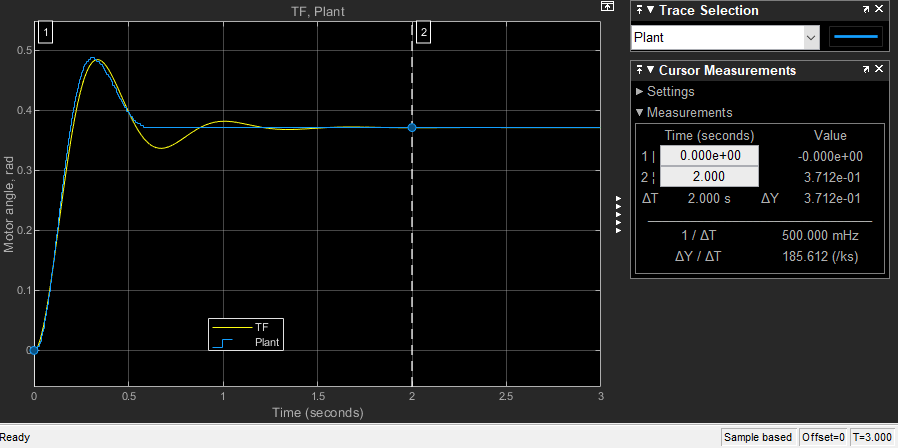
\includegraphics[width=9cm]{prac6_dc_gain_scope_step.PNG}
	\caption{Comparison of the transfer function and plant to a step input.}
\end{figure}  
\end{enumerate}
\PORTFOLIO{Compare your TF and Plant step responses.}
\end{frame}

\begin{frame}{Transfer Function Assessment}
\begin{enumerate}
    \setcounter{enumi}{5}
	\item Compare the response of the transfer function and plant to a $0.5$Hz Sine wave (2 periods of oscillation per second), keeping the same $0.5$V amplitude. Compare the amplitude and phase of the two responses, and observe how the aforementioned nonlinearities affect the physical system.
\begin{figure}	
    \centering
	
\includegraphics[width=9cm]{prac6_dc_sine_tracking.PNG}
	\caption{Comparison of the transfer function and plant to a sine input.}
\end{figure}  
\end{enumerate}
\PORTFOLIO{Compare the time-domain response of the TF and Plant.}
\end{frame}

\begin{frame}{Transfer Function Assessment}
\begin{enumerate}
    \setcounter{enumi}{6}
	\item Repeat Step 6 with a $1$Hz Sine wave, adding the setpoint to the Scope. Observe the phase delay between the voltage-controlled input and the system response.
\begin{figure}	
    \centering
	
\includegraphics[width=6cm]{prac6_dc_sine_tracking_1hz.PNG}
	\caption{Comparison of the transfer function and plant with the $1$Hz sine input. The signal is incorrectly labeled as a setpoint; as the system is open loop, this is a control input.}
\end{figure}  
\end{enumerate}
\PORTFOLIO{Comment on the phase difference between the input voltage and output.}
\end{frame}

\begin{frame}{PID tuning law}

Given confidence in our transfer function, we can find an appropriate PID tuning law to attain our PID gains. 

Using the transform $\tau = 1/\omega_n$, and assuming $\lambda = 0.2\tau$ with negligible time delay, the CIMC PID gains are found in the following table. Recall the time constants relate to the gains by $K_i= \frac{K_p}{\TTi}$ and $K_d = K_p \TTd$.
	\begin{table}
				\centering
				\begin{tabular}{|c|c|c|}
					\hline
					 $K_p$ & $\TTi$ & $\TTd$\\
					\hline 
					$\displaystyle \frac{10\zeta}{k}$ & $\displaystyle\frac{2\zeta}{\omega_n}$ & $\displaystyle\frac{1}{2\zeta\omega_n}$\\
					\hline	
				\end{tabular}
				\caption{Chien IMC Tuning Law}
			\end{table}
\end{frame}

\begin{frame}{PID controller}
In this procedure you will take your PID controller from Practicals 3 or 4 and implement it around the pole-placement controller.
\begin{enumerate}
	\item Create a subsystem of your PID controller. 
\begin{figure}	
    \centering
	
\includegraphics[width=8cm]{prac6_TF_pid_subsystem.PNG}
	\caption{Creation of a Simulink subsystem by highlighting a region of the block diagram, right clicking, then creating from selection.}
\end{figure}  
\end{enumerate}
\end{frame}

\begin{frame}{PID controller}

\begin{enumerate}
    \setcounter{enumi}{1}
	\item Implement the PID controller, acting on the QUBE subsystem. 
\begin{figure}	
    \centering
	
\includegraphics[width=10cm]{prac6_TF_PID_PP_controller.PNG}
	\caption{Comparison of the setpoint and PID-controlled output.}
\end{figure}  
\end{enumerate}
\end{frame}

\begin{frame}{PID controller}
\begin{enumerate}
    \setcounter{enumi}{2}
	\item Assess the setpoint tracking of the pendulum to a $0.5$Hz and $1$Hz Sine wave with $0.5$V amplitude.
\begin{figure}	
    \centering
	
\includegraphics[width=5cm]{prac6_TF_pid_p5hz.PNG}\hfill
    
\includegraphics[width=5cm]{prac6_TF_pid_1hz.PNG}
	\caption{PID controller setpoint tracking for $0.5$Hz and $1$Hz.}
\end{figure}  
\end{enumerate}
\PORTFOLIO{Plot the sinusoidal setpoint tracking results.}
\PORTFOLIO{Do you expect this controller to be effective at all frequencies?}

\end{frame}

\begin{frame}{PID controller}
\begin{enumerate}
    \setcounter{enumi}{3}
	\item Perform a step response on the system with a $\pi/4$ setpoint. Note: the QUBE motor will struggle to attain a setpoint greater than $\pm\pi/4$ radians.
\begin{figure}	
    \centering
	
\includegraphics[width=8cm]{prac6_TF_pid_step_45}
	\caption{PID controller step response with a $45$ degree setpoint.}
\end{figure}  
\end{enumerate}
\PORTFOLIO{Plot the step response and comment.}
\PORTFOLIO{Do the step response characteristics change with setpoint?}
\end{frame}

\SUBCONCEPT{Theoeretical analysis}

\begin{frame}{Compound pendulum}
The theoretical model for the compound pendulum system is given by the transfer function
\[\frac{\theta_m(s)}{v_m(s)} = \frac{114.1}{s^2 + 5.248s+235.1}. \]
Suppose someone implements a poor low-pass filter in the electronics/hardware, say a low pass filter with a cutoff frequency of 10 rad/s. The transfer function with this filter is then
\[\frac{\theta_m(s)}{v_m(s)} = \frac{114.1}{s^2 + 5.248s+235.1}\frac{10}{s+10}. \]
This part does not use the hardware. In Part 3, you will \textbf{create a new Simulink block diagram} i.e. we will not reuse anything from Part 1 except the CUBE block. You will to add the problematic low-pass filter before or after the QUBE block, input a sine wave, and log the data using a scope. 
\end{frame}

\begin{frame}{Frequency analysis}
Based on this model of the compound pendulum, use MATLAB to plot the Bode and Nyquist curves. You will need to enter the transfer function with the low-pass filter as the transfer function myTF. 

This has a similar notation to what we are used to within the Simulink Transfer Function block. When in doubt, right-click on \texttt{tf}, then click help.

\includematlab{prac6.m}{part1} 

Inspect the plots to identify regions of interest and consider which range of frequencies should be sampled.

\PORTFOLIO{Show both sets of Bode and Nyquist plots.}
\PORTFOLIO{What effect is the low-pass filter having on the system?}

\end{frame}

\SUBCONCEPT{Experimental analysis}

\begin{frame}{Frequency analysis}
The Bode and Nyquist curves can all be constructed from knowledge of the phase and amplitude of the output signal of a plant driven at a range of harmonic input frequencies. 

\begin{itemize}
	\item The code on the following slides will produce points on the prior Bode and Nyquist diagrams to compare these experimental results with the previously plotted theoretical plots
	\item You will need to provide the name of your Simulink model, a range of frequencies (around 10 different frequencies in rad/s) to run the system at, and the name of your input and output signals as given by the Scope logging variable in Simulink
	\item Using knowledge of how the Bode and Nyquist plots are constructed (such as in the lecture notes), fill in the places in the code surrounded by <> to populate your experimental points on the curves
\end{itemize}

Run the code with 1 or 2 frequencies to start with, to ensure you have configured the code and the MATLAB-Simulink interface correctly. Set the amplitude to $1$V and ensure you have an open loop system response.
\end{frame}

\begin{frame}{Frequency analysis}
	\includematlab{prac6.m}{part2} 
\end{frame}

\begin{frame}{Frequency analysis}
\includematlab{prac6.m}{part3} 
\end{frame}

\begin{frame}{Experimental plots}
You should receive something that looks similar to the below plots.
\begin{figure}
	\centering
	\includegraphics[width=\linewidth]{prac6_experimental}
\end{figure}
\PORTFOLIO{Show 10-30 experimental data points on both the Bode and Nyquist plots.}
\PORTFOLIO{How closely do the results align with the Bode and Nyquist plots?}

\end{frame}


\begin{frame}{System characteristics}
These plots provide us with a wealth of information of our system, such as 
\begin{itemize}
	\item Resonant frequency, $\omega_r$
	\item Stability 
	\item Gain margin, $GM$
    \item Phase margin, $PM$
\end{itemize}
Determine these properites of the system by reading their definitions in the lecture notes.

\PORTFOLIO{Tabulate $\omega_r$, $GM$, $PM$, and state whether the system is stable.}

\end{frame}


\begin{frame}{Next week}
	This week you theoretically and experimentally analysed the frequency response of the compound pendulum system using Bode and Nyquist plots. 
	
	This concludes the standard practical topics using the QUBEs and next week we will begin the practical project using the ping pong rig.
\end{frame}



\end{document}
